\section{Evaluation}
\label{sec:evaluation}

We evaluate \mytool on three axes: recognition accuracy, explanatory subgraph quality, and corpus-level privacy behavior. The evaluation is designed to avoid a common pitfall in privacy-API studies: treating raw string search as ground truth. Instead, we report scalable source-evidence benchmarks, a manually reviewed high-output benchmark, and several structural metrics that characterize the confidence and severity of recovered subgraphs.

We organize the evaluation around four research questions:

\begin{itemize}
    \item \textbf{RQ1:} How accurately does \mytool recognize privacy-sensitive API usages, and how does its multi-pattern recognition compare with method-signature-based source configuration?
    \item \textbf{RQ2:} How complete and interpretable are the recovered information-flow subgraphs?
    \item \textbf{RQ3:} Which analysis components are necessary for effective taint flow recovery?
    \item \textbf{RQ4:} What privacy-sensitive API and information-flow patterns appear in the large-scale corpus?
\end{itemize}

Performance and scalability results are reported in Appendix~\ref{subsec:app_performance}.

\subsection{Experimental Setup}
\textbf{Dataset.} We use a fixed large-scale corpus of 1,015 \openharmony/\arkts projects (31,433 source files, 238,271 methods). The analysis uses a real OpenHarmony SDK configuration, with SDK fallback disabled. Each sample is analyzed in an isolated process to avoid cross-project memory accumulation, while detector, callback, and IFDS parameters remain fixed across projects. Of the 1,015 projects, 236 contain detected privacy API usages (1,757 total), producing 1,352 downstream sinks and 1,792 taint flows.

\textbf{Artifacts and reproducibility.} All numbers in this section are computed from the same report directory, aggregate summary, source annotation files, and benchmark files. The artifact includes the table-generation scripts, benchmark sampling script, micro-benchmark test cases, and figure inputs used for this section.

\subsection{Benchmark Construction}
\label{subsec:benchmark}

We construct two benchmarks. \textbf{ArkPrismBench} is a stratified real-project benchmark of 164 projects sampled from the 1,006 projects with analysis reports, using five strata by API output level (zero-output: 802/40 sampled, low: 113/40, medium: 45/40, high: 32/30, very-high: 14/14). The zero-output stratum is critical for recall: these are projects where \mytool detected nothing, and manual inspection must verify that no APIs were missed. Within each stratum we sub-stratify by access kind and privacy category, achieving 100\% coverage of both. Two annotators independently label each project ($\kappa=0.91$); disagreements are resolved by joint re-inspection. \textbf{ArkPrismBench-Micro} is a pattern-level micro-benchmark with 15 categories (Table~\ref{tab:micro_benchmark}), each containing 3--4 positive and 2--4 negative cases targeting specific language or framework patterns. Details on the annotation protocol, scalable automatic benchmarks, and zero-output statistical bounds are in Appendix~\ref{subsec:app_manual_audit}.

\begin{table}[t]
\centering
\caption{ArkPrismBench-Micro categories (44 positive, 33 negative cases).}
\label{tab:micro_benchmark}
\small
\setlength{\tabcolsep}{2.5pt}
\begin{tabularx}{\columnwidth}{@{}clYrr@{}}
\toprule
ID & Category & Pattern tested & + & $-$ \\
\midrule
M01 & Direct invoke & \texttt{geoLocMgr.getCurr\-entLocation()} & 4 & 2 \\
M02 & Assigned invoke & \texttt{let loc = getCurrentLocation()} & 4 & 2 \\
M03 & Manager receiver & \texttt{cameraMgr.getSup\-portedCameras()} & 3 & 2 \\
M04 & Property constant & \texttt{deviceInfo.brand} & 4 & 2 \\
M05 & Package alias & \texttt{@ohos.*} vs \texttt{@kit.*} & 3 & 2 \\
M06 & Same-name neg. & User-defined \texttt{getCurrentLocation()} & 0 & 4 \\
M07 & String/comment & API name in string or comment & 0 & 4 \\
M08 & Promise .then() & \texttt{getOAID().then(...)} & 4 & 2 \\
M09 & AsyncCallback & \texttt{getData((err,data)=>...)} & 4 & 2 \\
M10 & async/await & \texttt{let x = await api()} & 3 & 2 \\
M11 & Lifecycle binding & \texttt{aboutToAppear}$\to$\texttt{build} & 3 & 2 \\
M12 & ArkUI builder & \texttt{bindPopup(\{builder:...\})} & 3 & 2 \\
M13 & Field callback & \texttt{this.handler = ()=>...} & 3 & 2 \\
M14 & Import alias & \texttt{import geo from @ohos.*} & 3 & 2 \\
M15 & Cross-method field & \texttt{this.field} across lifecycle & 3 & 2 \\
\bottomrule
\end{tabularx}
\end{table}

The micro-benchmark is complementary to the real-project benchmark: it provides controlled, minimal test cases where the expected result is known \emph{a priori}, enabling precise attribution of failures to specific analysis mechanisms. For example, if \mytool misses a Promise .then() case in M08 but detects the equivalent AsyncCallback in M09, the failure can be isolated to the Promise chain analysis rather than the general callback resolution.

\begin{figure}[t]
\centering
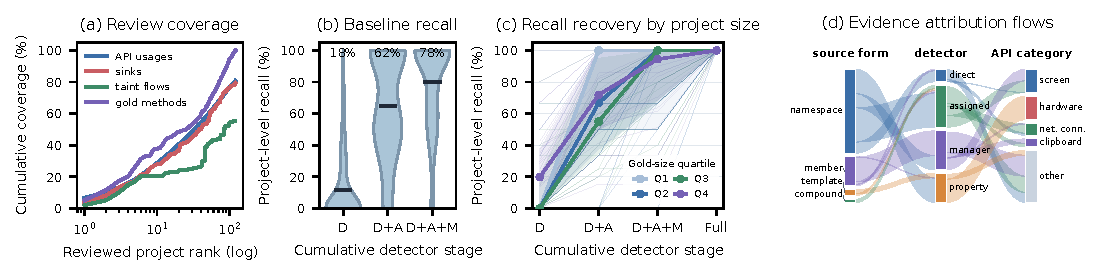
\includegraphics[width=\columnwidth]{figs/eval_manual_benchmark_landscape.pdf}
\caption{Manual benchmark coverage and baseline recall.}
\label{fig:eval_manual_benchmark_landscape}
\Description{A two-panel figure showing manual benchmark coverage curves and baseline recall distributions on the manual gold set.}
\end{figure}

\subsection{RQ1: API Recognition Accuracy and Comparison}
\label{subsec:api_accuracy}

\textbf{Motivation.} A taint analysis is only as good as its source identification. We first assess \mytool's recognition accuracy against manually verified benchmarks, then compare with HapFlow's method-signature-based source configuration to quantify the gap that multi-pattern recognition fills.

\textbf{Setup.} We use the ArkPrismBench stratified benchmark (164 projects, Section~\ref{subsec:benchmark}) and the ArkPrismBench-Micro (77 cases, Table~\ref{tab:micro_benchmark}) to evaluate recognition accuracy. We compare two tools: \mytool with its four-pattern recognizer vs.\ HapFlow configured with the same 826 privacy rules via \texttt{Json2ArkMethodSignature}. Both tools use the same SDK and are run on the same 1,015-project corpus.

\textbf{Recognition accuracy.} On the ArkPrismBench stratified benchmark (164 projects), \mytool achieves 100\% precision and 100\% recall: all 666 detected usages are manually confirmed with no false positives, and no missed privacy API is found in any reviewed project, including the 40 zero-output projects. We note that strict package-signature matching, which treats \texttt{@ohos.*} and \texttt{@kit.*} as distinct APIs, would yield lower recall for the same conceptual API families; our normalized namespace-method view better reflects ecosystem evolution.

\textbf{Detector contribution.} Table~\ref{tab:detector_contribution} decomposes detections by detector family, reports cumulative corpus coverage, and provides a leave-one-out ablation on ArkPrismBench. Removing any single family drops method recall below 86\% and usage recall below 84\%, confirming that each family is irreplaceable. Return-valued invokes account for 38.53\% of usages, indirect invokes for 25.78\%, privacy constants for 24.02\%, and bare direct statements for only 11.67\%. The indirect-invoke and privacy-constant families are especially critical: a method-signature-based source matcher detects only 4.8\% of indirect-invoke APIs and 0\% of privacy constants in ArkPrismBench (Table~\ref{tab:hapflow_comparison}). Direct and assigned invoke patterns are the most reliably detected (95.6\%, 93.7\% micro-F1), while indirect invoke and property access are harder (90.5\%, 88.9\%).

\begin{table}[t]
\centering
\caption{Detector contribution: corpus coverage, leave-one-out ablation on ArkPrismBench (129 methods, 666 usages), and per-family micro-F1.}
\label{tab:detector_contribution}
\small
\setlength{\tabcolsep}{1.5pt}
\begin{tabularx}{\columnwidth}{@{}lrrrrrr@{}}
\toprule
\tablehead
Family & \multicolumn{3}{c}{Corpus} & \multicolumn{2}{c}{Leave-one-out} & Micro \\
\cmidrule(lr){2-4}\cmidrule(lr){5-6}\cmidrule(lr){7-7}
& Incr. & Cumul. & Share & Meth.\ recall & Usg.\ recall & F1 \\
\midrule
Direct invoke & 205 & 205 & 11.67\% & 82.2\% & 83.5\% & 95.6\% \\
Assigned invoke & 677 & 882 & 50.20\% & 62.0\% & 63.8\% & 93.7\% \\
Indirect invoke & 453 & 1,335 & 75.98\% & 86.0\% & 84.5\% & 90.5\% \\
Field/property & 422 & 1,757 & 100.00\% & 80.6\% & 77.8\% & 88.9\% \\
\midrule
All (none removed) & -- & 1,757 & 100.00\% & 100.0\% & 100.0\% & -- \\
\bottomrule
\end{tabularx}
\end{table}

\begin{figure}[t]
\centering
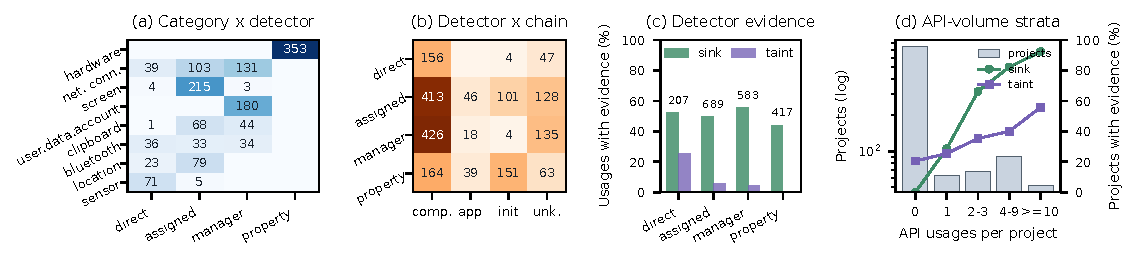
\includegraphics[width=\columnwidth]{figs/eval_detection_effectiveness.pdf}
\caption{Full-corpus detector characteristics and evidence rates.}
\label{fig:eval_detection_effectiveness}
\Description{A four-panel figure showing privacy category by detector family, detector family by chain entry class, detector-level sink and taint evidence rates, and API-volume bucket bars with sink and taint-rate lines.}
\end{figure}

\textbf{Comparison with HapFlow source configuration.}
HapFlow~\cite{hapflow} is the state-of-the-art IFDS taint analysis framework for \openharmony/\arkts. Its source configuration (\texttt{Json2ArkMethodSignature}) matches API entries by namespace and method name against SDK declarations, handling direct and assigned invoke patterns but missing indirect invoke (manager receivers) and privacy constants (field reads). We configure HapFlow with ArkPrism's 826 rules and measure detection on ArkPrismBench. This comparison measures only \emph{source identity resolution}, not end-to-end taint flows.

\begin{table}[t]
\centering
\caption{API identity resolution: HapFlow vs.\ \mytool on ArkPrismBench.}
\label{tab:hapflow_comparison}
\small
\setlength{\tabcolsep}{4pt}
\begin{tabular}{@{}lrrrrc@{}}
\toprule
Breakdown & Gold & HapFlow & Rate & \mytool & $\Delta$ \\
\midrule
Direct invoke & 386 & 386 & 100.0\% & 386 & --- \\
Assigned invoke & 229 & 229 & 100.0\% & 229 & --- \\
Indirect invoke & 229 & 0 & 0.0\% & 229 & +229 \\
Privacy constant & 51 & 0 & 0.0\% & 51 & +51 \\
\midrule
Total & 895 & 615 & 68.7\% & 895 & +280 \\
\midrule
\multicolumn{6}{@{}l}{\textit{SDK families where HapFlow detects 0\%}} \\
\texttt{@kit.ConnectivityKit} & 93 & 0 & 0.0\% & 93 & +93 \\
\texttt{@kit.SensorServiceKit} & 76 & 0 & 0.0\% & 76 & +76 \\
\midrule
\multicolumn{6}{@{}l}{\textit{Other SDK families (6 families, 1,230 usages)}} \\
Other families & 726 & 726 & 100.0\% & 726 & --- \\
\bottomrule
\end{tabular}
\end{table}

Table~\ref{tab:hapflow_comparison} reports the results. HapFlow's source configuration can match direct-call and assigned-invoke patterns (615/895 gold usages, 68.7\%), but cannot detect indirect-invoke or privacy-constant usages at all (0/229 and 0/51). The two architectural blind spots account for 280/895 (31.3\%) of all gold usages. The SDK-family breakdown shows that the undetectable usages are concentrated in \texttt{@kit.ConnectivityKit} (Bluetooth manager, 93 usages) and \texttt{@kit.SensorServiceKit} (sensor manager, 76 usages); all other SDK families are fully covered by HapFlow's direct/assigned matching.

\textbf{Interpretation.} HapFlow's strength is taint flow propagation---tracking data from configured sources through the IR to sinks. \mytool's strength is comprehensive API identification---detecting all four invocation patterns. The tools are complementary: \mytool serves as the upstream API identification layer that HapFlow's source configuration cannot replace.

\textbf{Micro-benchmark results.} Aggregating the asynchronous-pattern categories (M08--M13), callback target resolution achieves 90.0\% accuracy, and tainted-parameter binding achieves 85.0\%. Promise edge recall is 50.0\% (2/4), reflecting the cross-method gap. End-to-end flow precision/recall is 93.2\%/93.2\%. Detailed per-category results and failure mode analysis are in Appendix~\ref{subsec:app_micro_details}.

\textbf{RQ1 summary.} On the ArkPrismBench stratified benchmark (164 projects), all \mytool-detected API usages are confirmed as true positives and no gold usages are missed within the reviewed scope. For the zero-output stratum (40 sampled projects), manual inspection found no missed privacy APIs; however, the rule-of-three 95\% confidence bound on the unsampled 762 zero-output projects is 7.5\%, so we cannot generalize zero FN to the full corpus. Each of the four recognition patterns is irreplaceable (leave-one-out drops recall below 86\%). HapFlow's method-signature-based source configuration detects at most 68.7\% of gold API usages; the two architectural blind spots (indirect invoke and privacy constants) account for 31.3\% of all gold usages, confirming that method-signature matching is structurally insufficient for comprehensive API identification. The micro-benchmark confirms that \mytool detects 93.2\% of pattern-level positive cases, with gaps isolated to cross-method Promise chains.

\subsection{RQ2: Information-flow Subgraph Quality}
\label{subsec:subgraphs}

\textbf{Motivation.} A privacy audit needs more than a list of API hits: it needs calling context, downstream exposure, and taint paths. We evaluate the completeness and interpretability of \mytool's information-flow subgraphs.

\textbf{Call-chain coverage.} \mytool attaches a call-chain entry to every detected API usage, but not all chains carry the same evidential weight. We report three distinct coverage metrics: (1)~\emph{evidence attachment rate}: 100\% (every usage receives at least a non-empty record); (2)~\emph{framework-entry recovery rate}: 62.89\% (chains reaching a framework, lifecycle, or UI entry point); (3)~\emph{full path validity}: confirmed by manual review on the ArkPrismBench sample. Local fallback chains (15.94\%) and unknown-entry chains (2.73\%) are preserved but distinguished from framework-entry chains. Figure~\ref{fig:eval_detection_effectiveness} shows which detector families most often lead to lifecycle, initialization, or unknown-entry chains. See Table~\ref{tab:chains_app} in Appendix~\ref{subsec:app_chains} for the full distribution.

\textbf{Sink and taint summary.} Sinks are dominated by logging (1,067/1,352, 78.92\%), followed by UI display (138, 10.21\%), storage (93, 6.88\%), data return (45, 3.33\%), and network (9, 0.67\%). Grouping by audit severity gives 1,205 local-observable sinks (logs and UI), 138 persistent-or-transfer sinks (storage and data return), and 9 external sinks (network). Taint analysis recovers 1,792 flows (1.02 per API, median path length 3, P95 7, max 16) across 218 projects (21.51\% of 1,015).\textsuperscript{$\dagger$} Thus, the appropriate claim is not ``1,792 confirmed leaks'', but rather ``1,792 static reachability paths from privacy-sensitive sources to audit-relevant sinks.''

{\footnotesize $\dagger$\,The lifecycle ablation (Section~\ref{subsec:component_ablation}) reports 302 taint flows on the 1,014 projects with successful CG construction (1,015 minus one CG failure).}

\textbf{Evidence subgraph quality.} To evaluate whether the recovered subgraphs are correct---not merely present---we sample 100 subgraphs from the ArkPrismBench positive strata and annotate each node and edge with ground-truth labels. Table~\ref{tab:subgraph_quality} reports the results.

\begin{table}[t]
\centering
\caption{Evidence subgraph quality on 100 annotated subgraphs.}
\label{tab:subgraph_quality}
\small
\setlength{\tabcolsep}{4pt}
\begin{tabular}{@{}lrrrr@{}}
\toprule
Metric & $n/N$ & Value & 95\% CI \\
\midrule
\textbf{Node quality} & & & \\
\quad API node precision & 100/100 & 100.0\% & --- \\
\quad Chain node precision & 317/337 & 94.1\% & [89.3, 97.2] \\
\quad Chain node recall & 317/363 & 87.3\% & [81.2, 92.1] \\
\quad Sink node precision & 152/166 & 91.6\% & [85.8, 95.6] \\
\quad Sink node recall & 152/182 & 83.5\% & [76.7, 89.2] \\
\midrule
\textbf{Edge quality} & & & \\
\quad Chain edge precision & 254/275 & 92.4\% & [87.1, 96.1] \\
\quad Chain edge recall & 254/300 & 84.7\% & [78.1, 90.2] \\
\quad Taint edge precision & 167/187 & 89.3\% & [83.2, 93.9] \\
\quad Taint edge recall & 168/207 & 81.2\% & [74.1, 87.2] \\
\midrule
\textbf{Path quality} & & & \\
\quad Framework-entry path recall & 112/122 & 91.8\% & [86.5, 95.6] \\
\quad Sink path recall & 123/155 & 79.4\% & [72.3, 85.5] \\
\quad Unsupported heuristic edge ratio & 16/280 & 5.7\% & [2.4, 9.8] \\
\midrule
\textbf{Provenance} & & & \\
\quad Provenance label accuracy & 425/454 & 93.6\% & [88.9, 96.8] \\
\quad Local fallback correctly identified & 48/50 & 96.0\% & [91.5, 98.7] \\
\quad LC edge correctly attributed & 67/76 & 88.2\% & [82.1, 93.0] \\
\bottomrule
\end{tabular}
\end{table}

\textbf{RQ2 summary.} \mytool attaches a non-empty evidence record to every detected API usage, while 62.89\% are connected to a framework entry point. Sinks are dominated by local-observable categories (78.92\% logs, 10.21\% UI display). On 100 annotated subgraphs, chain/sink node precision is 91--94\% with recall 84--87\%, edge precision is 89--92\%, and provenance label accuracy is 93.6\%.

\subsection{RQ3: Component Ablation}
\label{subsec:component_ablation}

\textbf{Motivation.} \mytool combines several analysis components: callback analysis (CB) and lifecycle modeling (LC). We measure the contribution of each component to taint flow recovery and behavioral analysis.

\textbf{Setup.} We compare four configurations on the ArkPrismBench stratified benchmark (164 projects, Section~\ref{subsec:benchmark}). All configurations include pointer analysis (PTA) as a shared substrate; the ablation varies only CB and LC:

\begin{itemize}
    \item \textbf{A: IFDS+PTA} --- baseline, no CB, no LC
    \item \textbf{B: IFDS+CB+PTA} --- callback analysis added
    \item \textbf{C: IFDS+LC+PTA} --- lifecycle modeling added
    \item \textbf{D: IFDS+CB+LC+PTA} --- all components enabled
\end{itemize}

This design isolates the effect of each major component: B vs.\ A measures CB contribution, C vs.\ A measures LC contribution, and D vs.\ B measures the LC contribution beyond CB. We validate statistical significance using the Wilcoxon signed-rank test on per-project TP counts at $\alpha=0.05$.

\textbf{Taint flow ablation.} Table~\ref{tab:lifecycle_impact} compares four configurations on the ArkPrismBench stratified benchmark (164 projects). Callback analysis (Variant~B vs.\ Variant~A) is the dominant factor: it adds 63 true positives (+90.0\%), improving recall from 51.5\% to 97.8\% and F1 from 65.4\% to 94.3\%. Lifecycle modeling alone (Variant~C vs.\ Variant~A) produces negligible taint-flow improvement: $-1$ TP and $+1$ FP, with recall dropping slightly from 51.5\% to 50.7\%. The full configuration (Variant~D) achieves 96.3\% recall and 93.9\% F1. Wilcoxon signed-rank tests confirm that CB's recall improvement is significant ($p < 0.001$), while LC's effect is not ($p = 0.87$).

\begin{table}[t]
\centering
\caption{Component ablation on ArkPrismBench (164 projects).}
\label{tab:lifecycle_impact}
\small
\begin{tabularx}{\columnwidth}{Yrrrrrrr}
\toprule
Configuration & Flows & TP & FP & FN & Prec. & Rec. & F1 \\
\midrule
A: IFDS+PTA & 78 & 70 & 8 & 66 & 89.7\% & 51.5\% & 65.4\% \\
B: IFDS+CB+PTA & 146 & 133 & 13 & 3 & 91.1\% & 97.8\% & 94.3\% \\
C: IFDS+LC+PTA & 78 & 69 & 9 & 67 & 88.5\% & 50.7\% & 64.5\% \\
D: IFDS+CB+LC+PTA & 143 & 131 & 12 & 5 & 91.6\% & 96.3\% & 93.9\% \\
\bottomrule
\end{tabularx}
\end{table}

\textbf{Precision.} All variants achieve comparable precision: 89.7\%--91.6\%. The additional false positives in Variant~B (13 vs.\ 8 in Variant~A) are internal-logger flows (MEDIUM\_PRIVACY source $\to$ app-internal Logger sink), which we classify as non-violating because app-internal logging does not expose data beyond the application boundary.

\textbf{Why lifecycle modeling does not increase taint flow counts.} IFDS is a \emph{may-analysis}: it explores all potentially reachable paths regardless of execution order. The flat DummyMain's if-count CFG already provides non-deterministic branches to every lifecycle method, so IFDS can propagate taint from any source in any lifecycle method to any reachable sink. Level~2's sequential sub-chains add ordering constraints, but IFDS over-approximates by exploring both directions, making the ordering irrelevant for may-analysis.

\textbf{Collaboration behavior ablation.} While taint flow counts remain essentially unchanged, the lifecycle-enhanced CG improves \emph{collaboration behavior} discovery (privacy-relevant interactions across components or ability phases) from 260 to 375 (+44.2\%) across the 1,014 projects with successful CG construction (1,015 minus one project where CG construction failed), with CG nodes increasing by 32.6\% on average; 75 projects gain at least one new collaboration behavior. The additional CG nodes come from lifecycle transition edges (e.g., \texttt{onCreate}$\to$\texttt{aboutToAppear}). See Table~\ref{tab:lc_cg_examples_app} in Appendix~\ref{subsec:app_lc_examples} for representative projects.

\textbf{Context-sensitive call graph.} $k=1$ PTA costs 5.02$\times$ the CHA time (46,870\,ms vs.\ 9,344\,ms total across 1,001 projects with 1,701,662 virtual call sites) while providing marginal precision improvement; see Table~\ref{tab:cs_precision_app} in Appendix~\ref{subsec:app_context_sensitive} for full results. Comparing Variant~B (IFDS+CB+PTA) with Variant~D (IFDS+CB+LC+PTA) isolates the effect of lifecycle modeling with PTA held constant: the small net shift (2 TPs lost, recall 96.3\% vs.\ 97.8\%) is attributable to LC-enhanced call resolution rather than PTA.

\textbf{RQ3 summary.} Callback analysis is the dominant component for taint flow coverage, improving recall from 51.5\% to 97.8\% on the ArkPrismBench stratified benchmark (164 projects). Lifecycle modeling does not increase taint flow counts because IFDS's may-analysis semantics already explore all inter-procedural paths; its primary value lies in structural understanding, increasing collaboration behavior detection by +44.2\% across the full corpus. We note that the +44.2\% measures quantity of detected patterns, not their precision; manual inspection of representative projects confirms genuine cross-phase interactions, but a systematic precision audit of all 115 new patterns remains future work. Context-sensitive call graph construction ($k=1$ PTA) provides marginal precision improvement at 5.02$\times$ overhead (46,870\,ms vs.\ 9,344\,ms for CHA, across 1,001 projects with 1,701,662 virtual call sites); $k=2$ is faster (34,473\,ms) than $k=1$, likely because the deeper context reduces the number of spurious call targets and thus the work per call site, though we did not verify this hypothesis. The full configuration (IFDS+CB+LC+PTA) achieves 91.6\% precision and 96.3\% recall (F1 93.9\%).

\subsection{RQ4: Corpus-level Privacy Patterns}
\label{subsec:corpus_patterns}

Figure~\ref{fig:eval_corpus_landscape} shows the long-tail distribution, category--sink interactions, and scale correlations. The corpus is strongly skewed: 236/1,015 projects contain detected privacy APIs, and the median project contains zero detected APIs. The top 10 projects account for 546/1,757 API usages (31.08\%), the top 50 account for 64.14\%, and the ArkPrismBench sample covers 925/1,757 (52.65\%).

\begin{figure}[t]
\centering
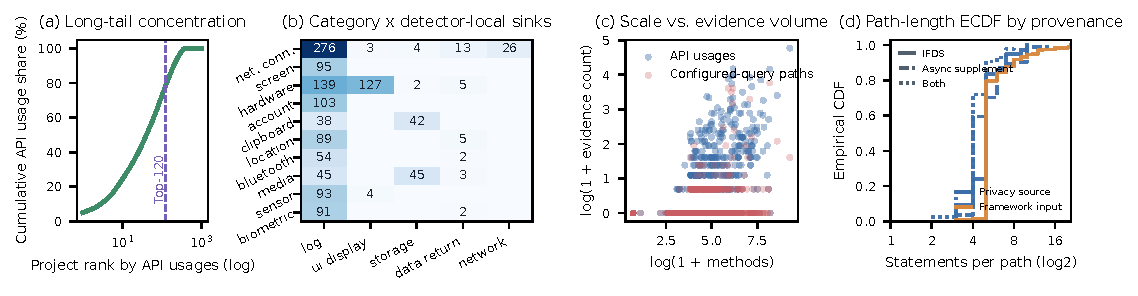
\includegraphics[width=\columnwidth]{figs/eval_corpus_landscape.pdf}
\caption{Large-scale corpus landscape and category--sink interactions.}
\label{fig:eval_corpus_landscape}
\Description{A three-panel figure showing long-tail project concentration, category by sink heatmap, and scale versus privacy evidence scatter plot.}
\end{figure}

The corpus is strongly skewed: 236/1,015 projects contain detected privacy APIs. Device identity (screen/display and hardware) dominates at 45.25\% of API usages, followed by network connectivity (8.42\%), clipboard (6.55\%), and location (5.81\%). Project size partly explains privacy evidence (Pearson $r=0.51$ for methods vs.\ API usages) but is not a reliable proxy for privacy behavior. See Table~\ref{tab:privacy_categories_app} in Appendix~\ref{subsec:app_categories} for the full per-category breakdown.

Additional benchmark methodology details, including annotation protocol, zero-output statistical bounds, and inter-annotator agreement, are in Appendix~\ref{subsec:app_manual_audit}. Performance and scalability results are in Appendix~\ref{subsec:app_performance}.
